% Created 2016-02-22 Mon 16:17
\documentclass[11pt]{article}
\usepackage[utf8]{inputenc}
\usepackage[T1]{fontenc}
\usepackage{fixltx2e}
\usepackage{graphicx}
\usepackage{grffile}
\usepackage{longtable}
\usepackage{wrapfig}
\usepackage{rotating}
\usepackage[normalem]{ulem}
\usepackage{amsmath}
\usepackage{textcomp}
\usepackage{amssymb}
\usepackage{capt-of}
\usepackage{hyperref}
\usepackage{minted}
\usepackage{minted}
\usemintedstyle{emacs}
\usepackage{mathrsfs,amsmath}
\usepackage[spanish]{babel}
\usepackage{subcaption}
\addto{\captionsspanish}{\renewcommand*{\contentsname}{Contenido}}
\renewcommand{\listingscaption}{Código}
\date{}
\title{}
\hypersetup{
 pdfauthor={},
 pdftitle={},
 pdfkeywords={},
 pdfsubject={},
 pdfcreator={Emacs 24.5.1 (Org mode 8.3.1)},
 pdflang={Spanish}}
\begin{document}

\newcommand{\set}[2]{\newcommand{#1}{#2}}
\newcommand{\materia}[1]{\set{\Cmateria}{#1}}
\newcommand{\tipo}[1]{\set{\Ctipo}{#1}}
\newcommand{\titulo}[1]{\set{\Ctitulo}{#1}}
\newcommand{\resumen}[1]{\set{\Cresumen}{#1}}
\tipo{Actividad 5}
\titulo{Receptor UART}
\materia{Verificacion de circuitos digitales}
\resumen{}
\set{\logoDeLaUniversidad}{/home/hao/dev/org/latex-plantilla/figures/UDG.png}
\set{\largoDelLogo}{7cm}
\set{\nombreDeLaUniversidad}{Universidad de Guadalajara}
\set{\nombreDelDepartamento}{Departamento de electrónica}
\set{\nombreDelAutor}{Eduardo Vazquez Diaz}
\set{\emailDelAutor}{lalohao@gmail.com}
\title{
  \textbf{\nombreDeLaUniversidad}\\
  \nombreDelDepartamento\\
  \begin{figure}[ht]
    \centering
    \includegraphics[width=\largoDelLogo]{\logoDeLaUniversidad}
  \end{figure}
  \textbf{\Ctipo{}}\\
  \Ctitulo{}\\
  \textit{\Cmateria{}}\\
}
\author{\nombreDelAutor{}\\\emailDelAutor{}}
\maketitle
\newpage
\tableofcontents
\newpage
\ifdef{\Cresumen}{
\begin{abstract}
  \Cresumen{}
\end{abstract}
}{}

\section{Objetivo}
\label{sec:orgheadline1}
Implementar un receptor UART estándar RS-232 en lenguaje de
descripción de hardware (\emph{verilog}) capaz de trabajar a 9600bps y
verificarlo.
\section{Introducción}
\label{sec:orgheadline2}
La comunicacion serial requiere dos señales \textbf{TxD} y
\textbf{RxD}. Usualmente se utiliza un conector de 9 pines (Figura \ref{fig:orgparagraph1}).

\begin{figure}[htb]
\centering
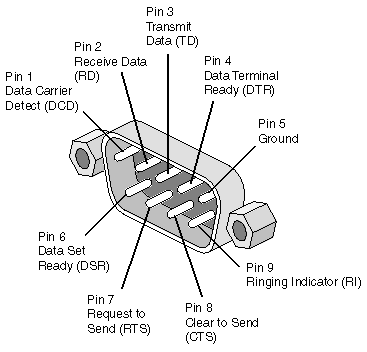
\includegraphics[width=7cm]{data/ee/9af60f-ed89-4c22-8d7b-e73cc7c9184d/screenshot-20160222-135017.png}
\caption{\label{fig:orgparagraph1}
Conector macho utilizado en el estandar RS-232}
\end{figure}

Los datos se transmiten a cierta velocidad conocida como \textbf{taza de
baudios} o \textbf{baud rate}. La velocidad esta dada en bits por segundo,
las mas comunes son 4800, 9600, 56000, 115200.

Existe ciertos bits \emph{especiales} utilizados para designar el inicio
y fin de la comunicación, como también lo hay para chequeo de
errores.

El bit de chequeo de error también se conoce como bit de paridad,
esta puede ser \textbf{par} o \textbf{impar} y se obtiene contando el numero de
\textbf{1} que contiene el dato, suponiendo que la paridad \textbf{par} esta
seleccionada y el numero de bits es impar entonces el bit de paridad
será 1. (Figura \ref{fig:orgparagraph2})

\begin{figure}[htb]
\centering
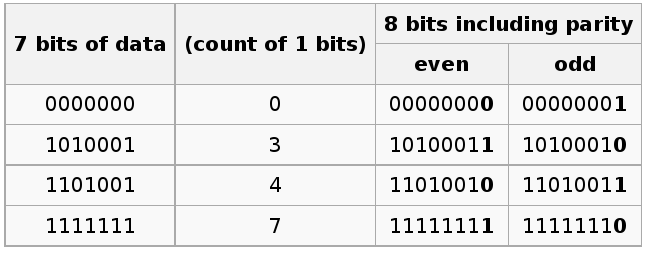
\includegraphics[width=.9\linewidth]{data/ee/9af60f-ed89-4c22-8d7b-e73cc7c9184d/screenshot-20160222-140423.png}
\caption{\label{fig:orgparagraph2}
Cálculo de paridad.}
\end{figure}

Una forma mas facil de calcular la paridad es aplicando el operador
modulo (Ecuación \ref{eq:paridad})

\begin{equation}\label{eq:paridad}
n\%2=p
\end{equation}

Sustituyendo \(n\) (el conteo de bits) se obtiene una paridad \(p\)
que es \textbf{par}, para la \textbf{impar} solo se invierte el bit.

La transmisión serial se sincroniza con los bits de inicio y los de
fin, normalmente se utiliza el código ASCII para comunicarse. Un
ejemplo de transmision de la letra \textbf{T} en codigo ASCII se da en la
figura \ref{fig:orgparagraph3}.

\begin{figure}[htb]
\centering
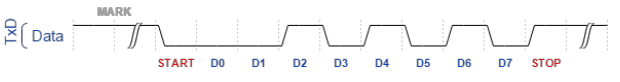
\includegraphics[width=.9\linewidth]{data/ee/9af60f-ed89-4c22-8d7b-e73cc7c9184d/screenshot-20160222-141608.png}
\caption{\label{fig:orgparagraph3}
ASCII 0x54 = 01010100 \textbf{T} enviado sin paridad.}
\end{figure}

\begin{figure}[htb]
\centering
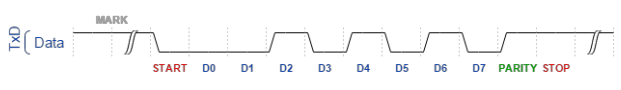
\includegraphics[width=.9\linewidth]{data/ee/9af60f-ed89-4c22-8d7b-e73cc7c9184d/screenshot-20160222-142005.png}
\caption{\label{fig:orgparagraph4}
ASCII 0x54 = 01010100 \textbf{T} con paridad \textbf{par}.}
\end{figure}

\begin{figure}[htb]
\centering
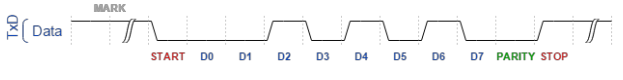
\includegraphics[width=.9\linewidth]{data/ee/9af60f-ed89-4c22-8d7b-e73cc7c9184d/screenshot-20160222-142042.png}
\caption{\label{fig:orgparagraph5}
ASCII 0x54 = 01010100 \textbf{T} con paridad \textbf{impar}.}
\end{figure}
\newpage
\section{Desarrollo}
\label{sec:orgheadline3}
Los datos entran de forma serial en \textbf{RxD} en cada ciclo de lectura y
se pasan al registro \textbf{rx\_data}, al finalizar la recepción tambien se
activa el bit \textbf{rdrf} (\emph{received data ready flag}).

\begin{figure}[htb]
\centering
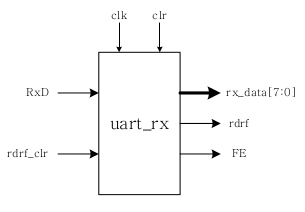
\includegraphics[width=7cm]{data/8d/f3fe04-f74c-41ea-a9f8-72c4f5d1492c/screenshot-20160222-142235.png}
\caption{Diagrama de bloques del receptor UART.}
\end{figure}

El modulo se implementa como una maquina de estados, como se
muestra en la figura \ref{fig:orgparagraph6}.

\begin{figure}[htb]
\centering
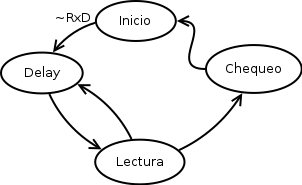
\includegraphics[width=7cm]{estados.png}
\caption{\label{fig:orgparagraph6}
Diagrama de estados del receptor UART.}
\end{figure}

El reloj funciona a una velocidad de 50Mhz, por lo que se utiliza un
retraso (delay) para sincronizar la señal a 9600bps diviendo el
reloj de 50Mhz entre 5208.

$$\frac{50,000,000}{5208}=9600.61443932$$

Durante el estado de inicio o reposo, la entrada \textbf{RxD} esta en
\emph{alto}, la comunicación empieza cuando \textbf{RxD} cambia a \emph{bajo} o
\(0\).

\begin{figure}[htb]
\centering
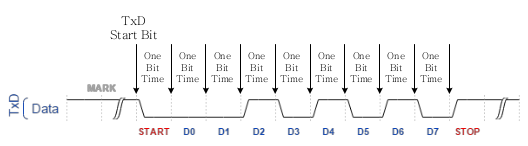
\includegraphics[width=.9\linewidth]{data/8d/f3fe04-f74c-41ea-a9f8-72c4f5d1492c/screenshot-20160222-154830.png}
\end{figure}

A partir de ese momento se va al estado de espera (\emph{delay}) hasta
que transcurre el tiempo suficiente y empiece a recibir el primer
dato, se repite el ciclo delay-recepción hasta que recibe todos los
bits de datos, paridad y stop.

En verilog se utilizaron 2 bloques \texttt{always}, el primero para manejar
la transición de estados y el segundo para dirigir las señales y
realizar las operaciones pertinentes.
\section{Resultados}
\label{sec:orgheadline4}
\begin{figure}[htb]
\centering
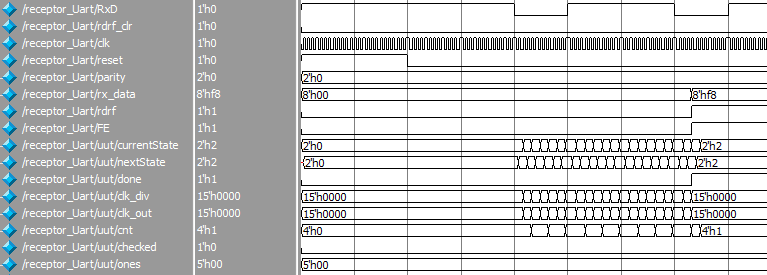
\includegraphics[width=.9\linewidth]{data/77/64c860-a96e-4031-b810-d94c6a7782e1/screenshot-20160222-160429.png}
\caption{Modulo receptor en funcionamiento.}
\end{figure}
\section{Conclusiones}
\label{sec:orgheadline5}
La verificación es una tarea esencial en el diseño de circuitos, en
este caso tuvo mayor complejidad que las tareas anteriores y se notó
que el uso de scripts pudieron haber facilitado la tarea.
\section{Apéndice}
\label{sec:orgheadline7}
\subsection{Código fuente}
\label{sec:orgheadline6}
\begin{minted}[]{verilog}
module receptor
  #(parameter DATA_LENGHT = 8,  // Datos de 8 bits
    parameter DELAY_TIME = 1)   // 50Mhz/5208=9600.61443932bps
   (input wire                   RxD,
    input wire                   rdrf_clr, clk, reset,
    input wire [1:0]             parity,
    output reg [DATA_LENGHT-1:0] rx_data,
    output reg                   rdrf, FE);

   reg [1:0]                     currentState, nextState;

   localparam START = 0, READ = 1, CHECK = 2, DELAY = 3; // Estados

   reg [DATA_LENGHT+1:0]         rx_data_tmp;      // Registro temporal de datos
   reg                           done;             // Bandera de finalizacion de lectura de datos
   reg [14:0]                    clk_div, clk_out; // Divisor de frecuencia
   reg [3:0]                     cnt;              // Contador de para recibir datos y parity check
   reg                           checked;          // Bandera de finalizacion de parity check
   reg [4:0]                     ones;             // Cuenta cuantos '1' existen
   reg                           parity_error;     // Bandera que designa error en paridad

   always @(posedge clk, posedge reset)
     if (reset)       currentState <= START;
     else             currentState <= nextState;

   always @(posedge rdrf_clr)
     rdrf <= 0;

   always @(posedge clk)                     // Control de estados
     case (currentState)
       START:
         if (RxD)     nextState = START;
         else         nextState = DELAY;
       DELAY:
         if (clk_out) nextState = READ;
         else         nextState = DELAY;
       READ:
         if (done)    nextState = CHECK;
         else         nextState = DELAY;
       CHECK:
         if (checked) nextState = START;
         else         nextState = CHECK;
     endcase // case (currentState)

   always @(currentState)                     // Flujo de datos
     case (currentState)
       START:
         begin
            {rx_data, rdrf, FE, ones} = 0;    // Poner senhales internas en cero
            {cnt, done, checked} = 0;         // Poner banderas en cero
            {clk_out, clk_div} = 0;           // Poner el divisor de frecuencia en cero
            parity_error = 0;
         end
       DELAY:
         begin
            clk_div = clk_div + 1;            // Divisor de frecuencia
            if (clk_div >= DELAY_TIME - 1)
              clk_out = 1;
         end
       READ:
         begin
            {clk_out, clk_div} = 0;           // Poner el divisor de frecuencia en cero
            rx_data_tmp[cnt] = RxD;           // Guardar dato

            cnt = cnt + 1;
            if (cnt > DATA_LENGHT + 1)
              begin
                 done = 1;
                 rdrf = 1;
                 cnt = 0;
                 rx_data = rx_data_tmp[7:0]; // Mover datos recibidos al registro Rx
                 if (~rx_data_tmp[9])        // Chequeo de stop bit
                   FE = 1;
              end
         end
       CHECK:
         begin
            ones = ones + rx_data[cnt];
            cnt = cnt + 1;
            if (cnt > DATA_LENGHT)
              begin
                 checked = 1;
                 if (parity == 2'b00 || parity == 2'b11) // No parity
                   parity_error = 0;
                 else if (parity == 2'b01)               // Even parity
                   parity_error = rx_data_tmp[DATA_LENGHT] == (ones % 2);
                 else                                    // Odd parity
                   parity_error = rx_data_tmp[DATA_LENGHT] == ~(ones % 2);
              end
         end
     endcase // case (currentState)

endmodule // receptor
\end{minted}
\end{document}
